% Annotated feedforward neural network for the data-driven-I lecture notebook.
%
% Same architecture as the figure it replaces (2 inputs, hidden layers
% of 3 and 4 neurons, 3 outputs, one bias neuron per layer) and the same style
% as the nn_* figures, but with everything labelled: layer names, bias neurons,
% the activation function rho, the weights/biases of each affine map, and the
% resulting composition.
%
% Build with:
%   latexmk -pdf neural_network_annotated.tex
%   pdftoppm -png -r 1200 neural_network_annotated.pdf tmp   % -> tmp-1.png, rename
%   latex neural_network_annotated.tex && dvisvgm --no-fonts --exact-bbox neural_network_annotated.dvi

\documentclass[11pt,border=2mm]{standalone}

\usepackage{amsmath}
\usepackage{tikz}
\usetikzlibrary{positioning,calc,decorations.pathreplacing}

\definecolor{pymor_blue}{HTML}{3155a0}
\definecolor{pymor_yellow}{HTML}{f0cf36}
\definecolor{DarkGray}{rgb}{0.274509804,0.254901961,0.235294118}

\tikzset{
  neuron/.style={circle, draw=pymor_blue, fill=white, text=DarkGray,
                 minimum size=0.66cm, inner sep=0pt, font=\small},
  bias/.style={neuron, draw=pymor_blue!60, fill=pymor_yellow!45},
  arrow/.style={->, >=stealth, draw=DarkGray!70, line width=0.35pt,
                shorten >=1pt, shorten <=1pt},
  biasarrow/.style={arrow, draw=pymor_yellow!85!black},
  title/.style={text=DarkGray, font=\small, align=center},
  maplabel/.style={text=DarkGray, font=\footnotesize},
  brace/.style={decorate, decoration={brace, amplitude=7pt, raise=5pt}, draw=DarkGray},
  note/.style={text=DarkGray, font=\footnotesize, align=left},
}

\newcommand{\vsep}{1.0}
\newcommand{\hsep}{2.9}
\newcommand{\ytop}{2.35}      % height of the layer titles
\newcommand{\ybias}{-2.45}    % height of the bias row
\newcommand{\ymap}{-3.35}     % height of the W/b labels

% #1 layer name, #2 count, #3 x, #4 node content prefix (empty for none)
\newcommand{\layer}[4]{%
  \foreach \i in {1,...,#2} {%
    \pgfmathsetmacro{\ypos}{-(\i - (#2+1)/2)*\vsep}%
    \node[neuron] (#1-\i) at (#3,\ypos) {$#4$};%
  }%
}
\newcommand{\layerindexed}[4]{%
  \foreach \i in {1,...,#2} {%
    \pgfmathsetmacro{\ypos}{-(\i - (#2+1)/2)*\vsep}%
    \node[neuron] (#1-\i) at (#3,\ypos) {$#4_{\i}$};%
  }%
}
% #1 source, #2 source count, #3 target, #4 target count
\newcommand{\connect}[4]{%
  \foreach \i in {1,...,#2} {\foreach \j in {1,...,#4} {\draw[arrow] (#1-\i) -- (#3-\j);}}%
}
% bias neuron #1 at x #2, connected to layer #3 with #4 neurons
\newcommand{\biasneuron}[4]{%
  \node[bias] (#1) at (#2,\ybias) {$1$};%
  \foreach \j in {1,...,#4} {\draw[biasarrow] (#1) -- (#3-\j);}%
}

\begin{document}
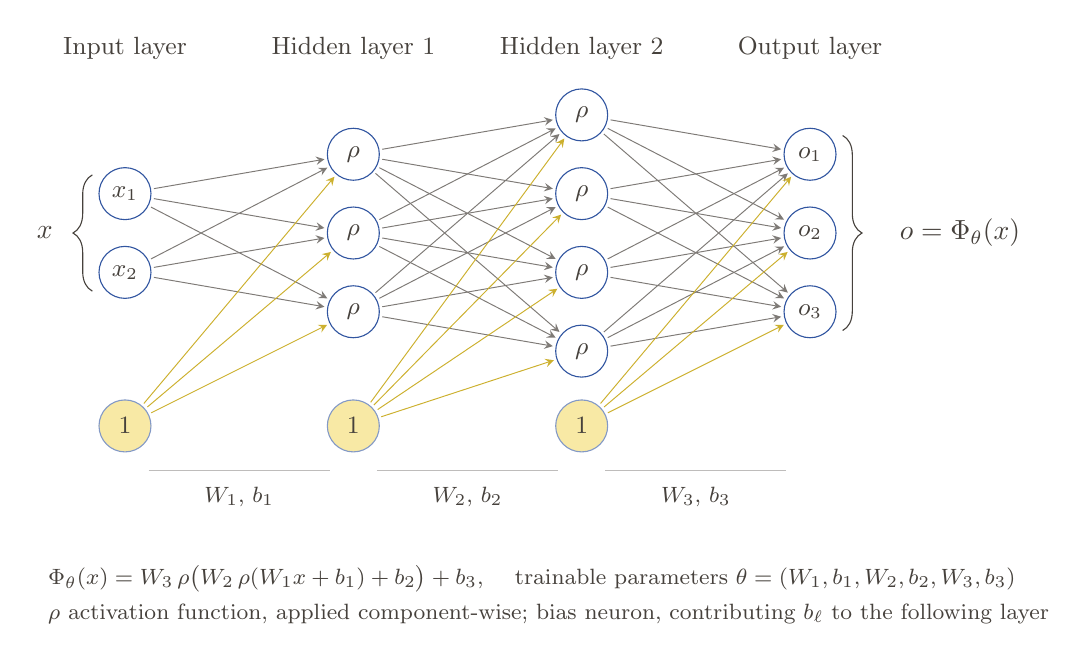
\begin{tikzpicture}

  % --- neurons -------------------------------------------------------------
  \layerindexed{input}{2}{0}{x}
  \layer{hiddenA}{3}{\hsep}{\rho}
  \layer{hiddenB}{4}{2*\hsep}{\rho}
  \layerindexed{output}{3}{3*\hsep}{o}

  % --- affine maps ---------------------------------------------------------
  \connect{input}{2}{hiddenA}{3}
  \connect{hiddenA}{3}{hiddenB}{4}
  \connect{hiddenB}{4}{output}{3}

  \biasneuron{bias-1}{0}{hiddenA}{3}
  \biasneuron{bias-2}{\hsep}{hiddenB}{4}
  \biasneuron{bias-3}{2*\hsep}{output}{3}

  % --- layer titles --------------------------------------------------------
  \node[title] at (0,\ytop) {Input layer};
  \node[title] at (\hsep,\ytop) {Hidden layer 1};
  \node[title] at (2*\hsep,\ytop) {Hidden layer 2};
  \node[title] at (3*\hsep,\ytop) {Output layer};

  % --- which weights act between which layers ------------------------------
  \node[maplabel] at (0.5*\hsep,\ymap) {$W_1,\,b_1$};
  \node[maplabel] at (1.5*\hsep,\ymap) {$W_2,\,b_2$};
  \node[maplabel] at (2.5*\hsep,\ymap) {$W_3,\,b_3$};
  \foreach \k in {0.5,1.5,2.5} {
    \draw[draw=DarkGray!35, line width=0.3pt]
      ($(\k*\hsep-1.15,\ymap+0.34)$) -- ($(\k*\hsep+1.15,\ymap+0.34)$);
  }

  % --- input / output braces ----------------------------------------------
  \draw[brace, decoration={mirror}] (input-1.north west) -- (input-2.south west)
    node[midway, xshift=-0.78cm, text=DarkGray] {$x$};
  \draw[brace] (output-1.north east) -- (output-3.south east)
    node[midway, anchor=west, xshift=0.78cm, text=DarkGray] {$o=\Phi_\theta(x)$};

  % --- legend and the resulting composition -------------------------------
  \node[note, anchor=north west] at (-1.1,\ymap-0.75)
    {$\Phi_\theta(x) = W_3\,\rho\big(W_2\,\rho(W_1x+b_1)+b_2\big)+b_3$,
     \quad trainable parameters $\theta=(W_1,b_1,W_2,b_2,W_3,b_3)$\\[3pt]
     $\rho$ activation function, applied component-wise;
     bias neuron, contributing $b_\ell$ to the following layer};

\end{tikzpicture}
\end{document}
